%%%%%%%%%%%%%%%%%%%%%%%%%%%%%%%%%%%%%%%%%%%%%%%%%%%%%%%%%%%%%%%%%%%%%%%%%%%
%
%    phase1-AR.tex  (use only for Archival Research and Theory proposals; use phase1-GO.tex
%                     for General Observer and Snapshot proposals and phase1-DD.tex for GO/DD 
%                     proposals or use phase1-MC.tex for GO/MC rapid response proposals.
%                     
%
%    HUBBLE SPACE TELESCOPE
%    PHASE I ARCHIVAL & THEORETICAL RESEARCH PROPOSAL TEMPLATE 
%    FOR CYCLE 24 (2016)
%
%    Version 1.1, August 12,  2015.
%
%    Guidelines and assistance
%    =========================
%     Cycle 23 Announcement Web Page:
%
%         http://www.stsci.edu/hst/proposing/docs/cycle23announce 
%
%    Please contact the STScI Help Desk if you need assistance with any
%    aspect of proposing for and using HST. Either send e-mail to
%    help@stsci.edu, or call 1-800-544-8125; from outside the United
%    States, call [1] 410-338-1082.
%
%%%%%%%%%%%%%%%%%%%%%%%%%%%%%%%%%%%%%%%%%%%%%%%%%%%%%%%%%%%%%%%%%%%%%%%%%%%

% The template begins here. Please do not modify the font size from 12 point.

\documentclass[12pt]{article}
\usepackage{phase1}

\usepackage{graphicx}
%\usepackage{amssymb}

\usepackage{wrapfig}
\usepackage{setspace}
%\usepackage{subfigure}
\usepackage{subcaption}
\usepackage{mathtools}

\graphicspath{/Users/David/Research_Documents/inclination/git_inclination/pilot_paper_code/pilot_paper/paper_figures2/}

\begin{document}

%   1. SCIENTIFIC JUSTIFICATION
%       (see Section 9.1 of the Call for Proposals)
%
%
\justification          % Do not delete this command.
% Enter your scientific justification here.

%The majority of the baryons in the universe are found in the intergalactic medium (IGM). The properties of this important reservoir of matter are most directly measured via absorption in the spectra of UV-bright background QSOs. The UV initiatives undertaken by the Cosmic Origins Spectrograph on HST have produced a wealth of high resolution and high signal-to-noise spectra that are ideal for a wide variety of IGM studies. However, the identification and measurement of spectral features is a major undertaking, and limits the viability of large-scale studies using archival HST data. We propose to create a legacy data archive of all archival COS sightlines, complete with line identifications and measurements. In addition, we will match nearby ($cz \leq 10,000$ km/s) spectral features with probable associated galaxies using the likelihood method we have developed (French et al. 2016, in prep). This will be the first large, publicly accessible IGM absorber dataset, and will provide a legacy artifact directly in line with the NASA Mission Directive whatever-it's-call-thing.


%Galaxy evolution relies on the recycling of material between the star-forming interstellar medium and the cosmological gaseous filaments in which galaxies reside. The interplay of gas accretion and feedback into and from the intergalactic and circumgalactic media (IGM and CGM) is difficult to observe, yet crucial for understanding and modeling galaxy evolution throughout cosmic time. 

%Fortunately, important physical properties of the IGM and CGM can be measured by observing spectral absorption lines on the continuum of UV-bright background quasars. For example, QSO spectroscopy has shown that, for absorbing systems in galaxy haloes, the equivalent width (e.g. Bowen et al. 2002), linewidth (e.g. Wakker & Savage 2009), column density (e.g. Rudie et al 2012), and metallicity (e.g. Kacprzak et al. 2014) all decrease with the distance to the nearest bright galaxy.

%Nevertheless, many open questions remain concerning the details of how gas near galaxies, extending throughout CGM to twice the virial radius, interacts with and affects galaxy evolution. The key questions we will answer are: a) how do the properties of CGM absorbers (e.g. equivalent width, location, velocity) compare to the properties of the galaxies they are associated with (e.g. size, inclination, morphology)? b) does the CGM follow the rotation direction and velocity of the associated galaxies, as predicted by simulations (e.g. Stewart et al. 2011)?


\indent \indent Galaxies reside within large gaseous filaments, and they evolve through complex interactions with this surrounding medium (the intergalactic medium or IGM). This gas is enriched by material ejected from the galaxies, and the galaxies draw new material from it for continuing star formation. Studying these complex interactions observationally is challenging, yet of great importance for understanding and modeling global galaxy evolution.

%\indent \indent The majority of the baryons in the universe are found in the intergalactic and circumgalactic medium (IGM, CGM) (e.g. Lehner et al. 2007, Danforth $\&$ Shull 2008, Cen 2013 and references therein). Galaxies reside within large gaseous filaments, from which they draw new material for continuing star formation, and into which they eject enriched material. Observationally studying these complex interactions is challenging, yet paramount to properly understanding and modeling global galaxy evolution.

At least $30\%$ of this gas is in a cool ($T \sim 10^{3-5}$K) and diffuse phase, and thus can be detected and its properties measured as Ly$\alpha$ absorption in the spectra of UV-bright background QSOs (Werk et al. 2014). Studies using this method have found numerous IGM-galaxy proximity effects, such as absorption equivalent width (e.g. Bowen et al. 2002), linewidth (e.g. Wakker $\&$ Savage 2009), column density (e.g. Rudie et al 2012), and metallicity (e.g. Kacprzak et al. 2014) decreasing with the distance to the nearest bright galaxy. 

%(the CGM, generally considered to extend to $\sim 2R_{vir}$)

Nevertheless, many open questions remain concerning the details of how the circumgalactic medium (CGM, the gas within $\sim 2R_{vir}$ of a galaxy) interacts with and affects galaxy evolution. The key questions we will answer are:
a) how do the properties of CGM absorbers (e.g. equivalent width, location, velocity) compare to the properties of the galaxies they are associated with (e.g. size, inclination, morphology)?
b) does the CGM follow the rotation direction and velocity of the associated galaxies, as predicted by simulations (e.g. Stewart et al. 2011)?

More generally, we would like to know whether galaxies shape their environments or vice-versa. Studying the properties of neutral H\,{\sc i} via Ly$\alpha$ absorption is one of the most direct ways to probe the galaxy-IGM interface. A large sample of absorbers with associated galaxies will provide clues to inflow and outflow behavior, halo gas dynamics and composition, and how gas and galaxies are oriented and interact in a broader, cosmological context. To answer these questions it will be necessary to probe gas both very near as well as physically far from galaxies. This is most easily done in the nearby universe, where the galaxy sample is highly complete to low luminosities. However, previous studies have suffered from several shortcomings. We propose a program using archival COS data to deal with the following 3 issues in particular:\\


\noindent 1) \textbf{\underline{Galaxy Incompleteness}}: As the completeness of known galaxies decreases sharply with redshift, many CGM studies suffer from limitations due to inhomogeneous and incomplete galaxy data. For example, Mathes et al. (2014) and Werk et al. (2014) are only complete to $\sim$$L^{\**}$ (at $0.12<z<0.67$ and $z\sim$$0.2$, respectively). This complicates the process of associating absorption with nearby galaxies, and may result in significant biases. Additionally, very few galaxies have published rotation curves, so comparing the velocity of the gas in the CGM to that within the disks of the associated galaxies is usually not possible. Distant galaxies also tend to have less detailed information (e.g. inclination, position angle, size), and are more prone to misclassification.

\textbf{Our solution - A new galaxy catalog for the redshift range $cz \leq 10,000$ km/s:} In this range, available galaxy data is complete to $\sim0.2 L^{\**}$ at $10,000$ km/s (and better towards lower redshifts). We created this galaxy catalog by mining the NASA Extragalactic Database (NED), collecting redshifts, diameters, redshift-independent-distances, morphologies, inclinations, position angles, photometry, and more for each galaxy, and then normalizing these values beyond the basic work done by NED. This catalog is the most complete, comprehensive and up-to-date nearby galaxy catalog in existence (to be published in 2016), and is key to drawing direct comparisons between the properties of the absorbers in the CGM and the properties of galaxies on a larger scale then ever before.\\

%In order to correlate CGM absorber properties with a galaxy, a match must be made between a galaxy to an absorption feature, but it is often unclear or arbitrary how this matching is done. 

\noindent 2) \textbf{\underline{Reproducibility}}: It is often unclear and sometimes arbitrary how absorption features are matched with a galaxy. Some authors (e.g. Kacprzak et al. 2011) pick the galaxy closest to the detected IGM absorber, while others (e.g. Wakker $\&$ Savage 2009) try to take galaxy size and other properties into account, and most tend to deal with ambiguities in an ad-hoc manner. This makes it difficult to compare results between different studies, and is preventing us from building a more global picture of the galaxy-IGM connection.
%However, different authors continue to use different, subjective criteria, and tend to deal with ambiguities in an ad-hoc manner.

\textbf{Our solution - Likelihood Method: } In French $\&$ Wakker (2016, in prep) we are introducing a reproducible method to streamline these types of decisions. We define the likelihood as:

\begin{equation}
	\mathcal{L} = e^{-(\rho/R_{vir})^2} e^{-(\Delta v / 200)^2},
\end{equation}
where $\rho$ is the physical impact parameter between the sightline and a galaxy, $R_{vir}$ is the galaxy's virial radius, and $\Delta v = v_{galaxy} - v_{absorber}$, the difference in velocity between the galaxy and the absorption line. In our pilot study (French $\&$ Wakker 2016, in prep, see below) we require $\mathcal{L}$ to be a factor of 5 larger than $\mathcal{L}$ for all other galaxies, and $\mathcal{L} \geq 0.001$, for a galaxy to be marked ``associated" with an absorption line. This hard limit translates to an absorber located at $\sim 2 R_{vir}$ and $\sim 350$ km/s in physical and velocity separation, respectively. This edge agrees with previous practice, but is rigorously defined (see Figure \ref{line} for an example). 

Furthermore, we can use this method as a tunable parameter, and break down our results into bins of likelihood. This allows us to study how, e.g., the equivalent width and $\Delta v$ of an absorber population evolve with stricter or more relaxed galaxy-association criteria.\\

% IGM-CGM border (e.g. Stocke et al. 2013 and Mathes et al. 2014).

\noindent 3) \textbf{\underline{Sample size}}: Probing the CGM in absorption requires a serendipitously-located background source, usually only one of which can be found for a particular galaxy. It is thus necessary to study the statistics of a large dataset of single galaxy-absorber matches. However, current CGM surveys max out at fewer than 100 galaxy-absorber pairs (e.g. 93 in Wakker $\&$ Savage 2009, 44 in Tumlinson et al. 2013, 89 in Steidel et al 2010, 71 in Stocke et al 2013).

\textbf{Our solution - 1) Archival data:} At the time of writing, 550 QSO targets have been observed with COS. Of the 300 with S/N$\geq$10, 120 have $0.03\leq z \leq 0.2$, such that intrinsic Ly$\alpha$ is in the G130M wavelength range, 90 have $0.2\leq z \leq 0.45$, putting Ly$\alpha$ in G160M, and 90 have $z > 0.45$. Nearly all of these pass within 500 physical kpc of at least one galaxy in the $cz \leq 10,000$ km/s redshift range. In our pilot study of 35 sightlines, we measured 176 Ly$\alpha$ absorption lines, 42 of which we paired with a nearby galaxy using our likelihood method. Hence, we predict 300 total spectra should produce over 1500 absorption lines and 360 absorber-galaxy pairings.

%\textbf{Our solution - 2) Line Identification}: The identification and measurement of spectral features is a major undertaking, and limits the viability of large-scale studies using archival HST data. To combat this we have developed a pipeline that helps automate the IDing of targets, which will allow us to produce a sample of hundreds of spectra and thousands of absorption lines. As the final step of our proposed program, we will create a legacy data archive of identifications and measurements of COS sightlines, complete with probable galaxy associations.\\

\textbf{Our solution - 2) Line Identification}: Identifying (IDing) and measuring spectral features for a large number of sightlines is extremely time-consuming, and generally limits the viability of large-scale studies like ours. To combat this we have developed a pipeline that helps automate the IDing of targets, which will allow us to produce a sample of hundreds of spectra and thousands of absorption lines. As the final step of our proposed program, we will create a legacy data archive of identifications and measurements of COS sightlines, complete with probable galaxy associations.\\

\noindent \textbf{\underline{Pilot Study:}}\\
\indent In French $\&$ Wakker (2016, in prep) we will present results from an initial study of 35 COS sightlines. This sub-sample yields 176 Ly$\alpha$ systems at $cz$ $\leq$ $10,000$ km/s, $32\%$ of which can be unambiguously paired with a single galaxy using our likelihood selection algorithm. In agreement with previous studies (e.g. Rudie et al 2012, Wakker $\&$ Savage 2009 and references therein), we find a steep increase in Ly$\alpha$ equivalent width ($W$) with decreasing impact parameter. However, normalizing for galaxy size produces a stronger correlation, so proximity is clearly not the only important factor (Figure \ref{virial}). Absorbers are also preferentially detected around highly inclined galaxies, with $73\%$ associated with a galaxy of inclination $>$ $50^{\circ}$. 

We also discovered a dichotomy in the equivalent width of absorption detected red-ward vs blue-ward of the systemic velocity of the associated galaxies (see Figure \ref{dichotomy}), with $\overline{W}$(redshifted) = 153$\pm$14 m\AA, and $\overline{W}$(blueshifted) = 321$\pm$13 m\AA~. This difference is significant at the $99\%$ level from results of both the Anderson-Darling and Kolmogorov-Smirnov statistical distribution tests. Following the suggestions of recent simulations (e.g. van de Voort et al. 2012), this could be evidence of cold, filamentary inflows, which are expected to be dense, and/or hot, lower density outflows. However, the robust statistics and increased parameter space of our proposed survey are necessary to fully explain these intriguing new results.\\

\noindent \underline{\textbf{Summary: }}\\
\indent Galaxies have a complex relationship with their environment, and are known to both eject and accrete material from the surrounding IGM. Although many studies have probed this CGM gas, none yet have overcome the issues of incompleteness, small sample size, and reproducibility. We propose a large scale survey to overcome these common shortcomings, and provide robust statistics on how the properties of Ly$\alpha$ absorption depend on the properties of nearby galaxies. We will select 300 of the 550 available COS sightlines to ID and cross-correlate with our nearby galaxy catalog, and produce the largest yet galaxy-absorber catalog. This will also provide a legacy dataset of ID'd and measured absorption lines for a majority of COS sightlines, which will continue to be useful to the community long after the end of this project.\\


%In attempt to combat these issues, we have begun a large scale survey of nearby COS sightline-galaxy associations, restricting ourselves to $cz \leq 10,000$ km/s, where we have assembled a galaxy catalog complete to $L^{\**}\sim 0.1$. To address the reproducibility issue, we have developed a probability algorithm to automatically choose which galaxy to associate an absorption line with. 
%
%Finally, we have been awarded priority 1 time on the Southern Africa Large Telescope (SALT) in order to measure the rotation curves of 15+ galaxies that have absorption detected in a sightline within 300 kpc and 400 km/s of the galaxy. This data combined with archival COS sightlines will allow us to finally probe how the kinematics of the CGM compare to that of the gas within the disks of galaxies.


%Studies of the circumgalactic medium, or the IGM-galaxy connection, generally rely on matching absorption measured in the spectra of background QSOs to a nearby foreground galaxy. The methods used for matching a galaxy to an IGM absorber are universally ad-hoc, however, and range from picking the nearest galaxy in physical impact parameter, to some combination of impact parameter, size, and judgement. 

%Other studies supplement archival galaxy data with new observations, but then the search radius is usually limited to a $<10'$ field of view. For example, Mathes et al. (2014) use imaging from the WFPC2 camera on HST, but their impact parameter limit is 300 kpc, close to the commonly accepted boundary between CGM and IGM gas (based on virial radii and/or escape velocity arguments, e.g., see Stocke et al. 2013 and Mathes et al. 2014). 


\begin{figure}[h!]
    \centering
    \begin{subfigure}[t]{0.5\textwidth}
        \centering
        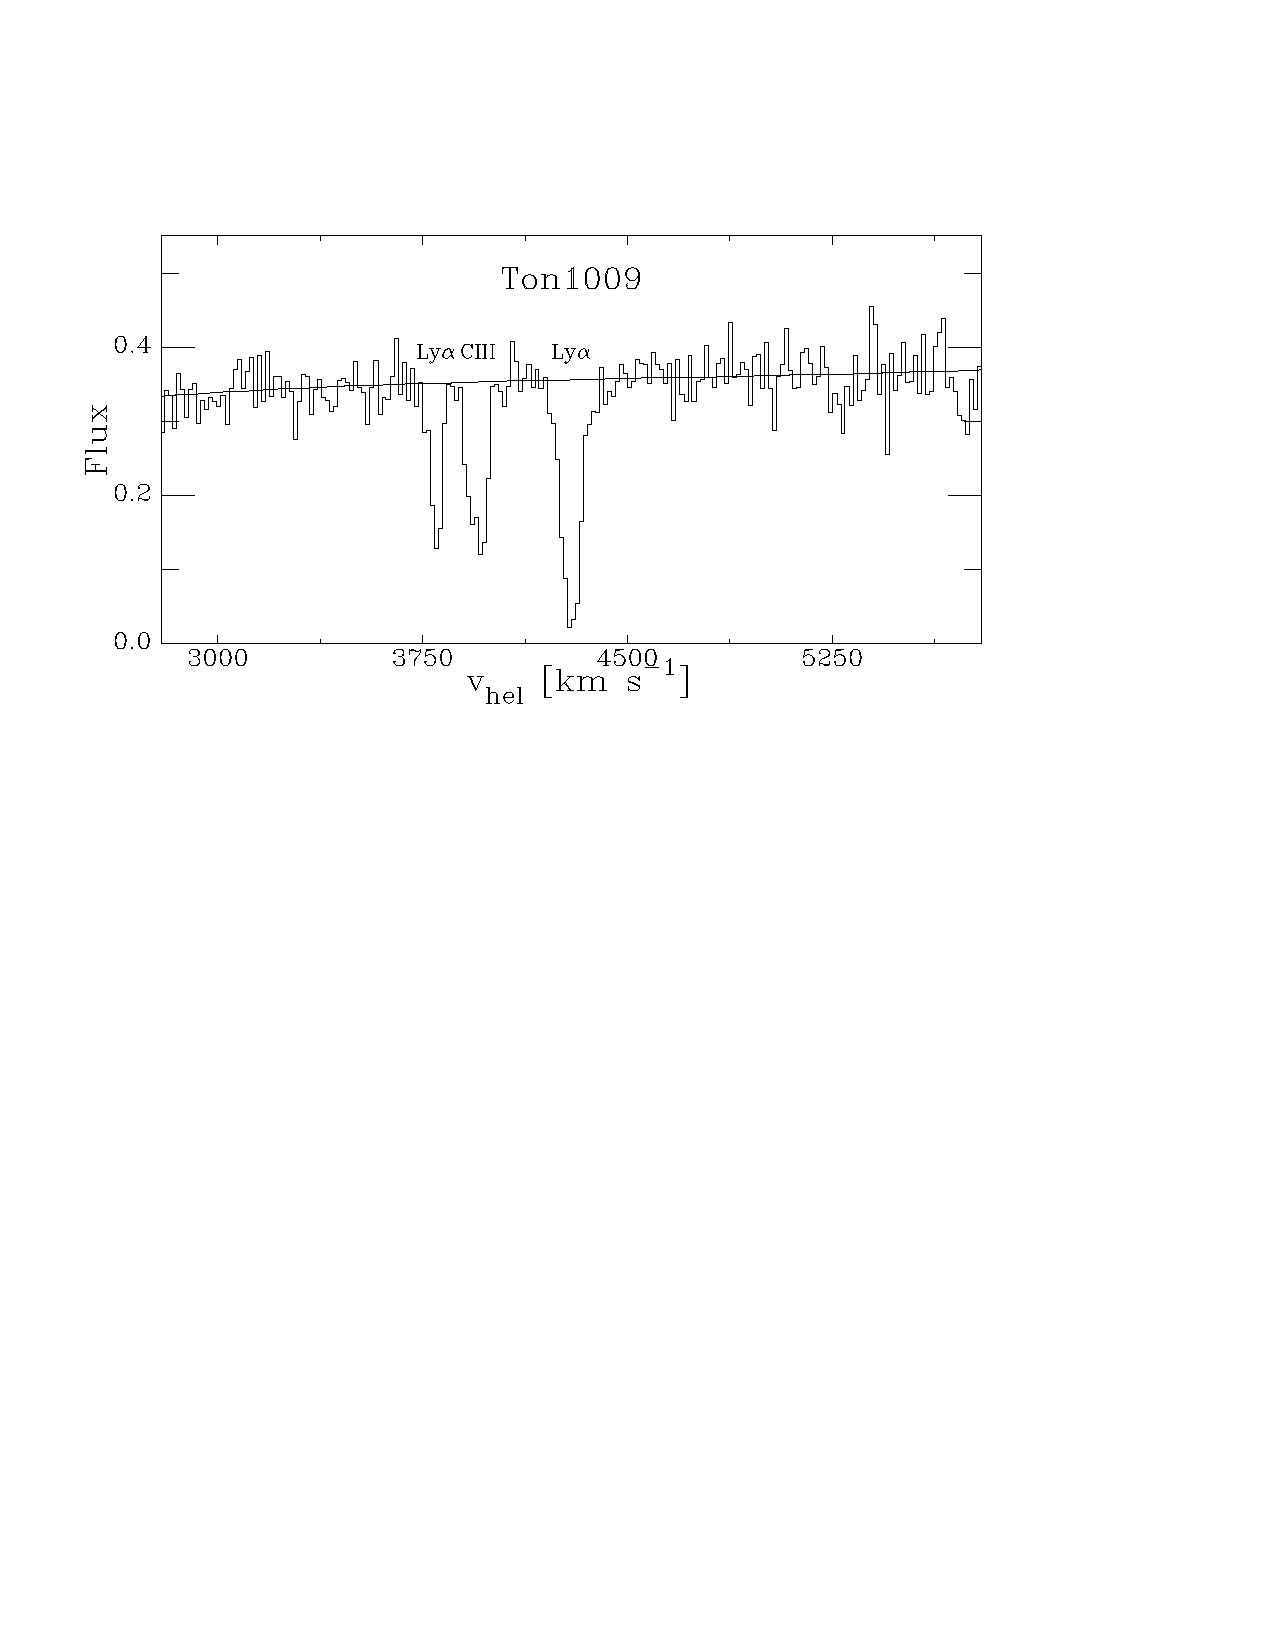
\includegraphics[width=\textwidth]{figTON1009_crop.pdf}
        \caption{}
    \end{subfigure}%
    ~ 
    \begin{subfigure}[t]{0.5\textwidth}
        \centering
        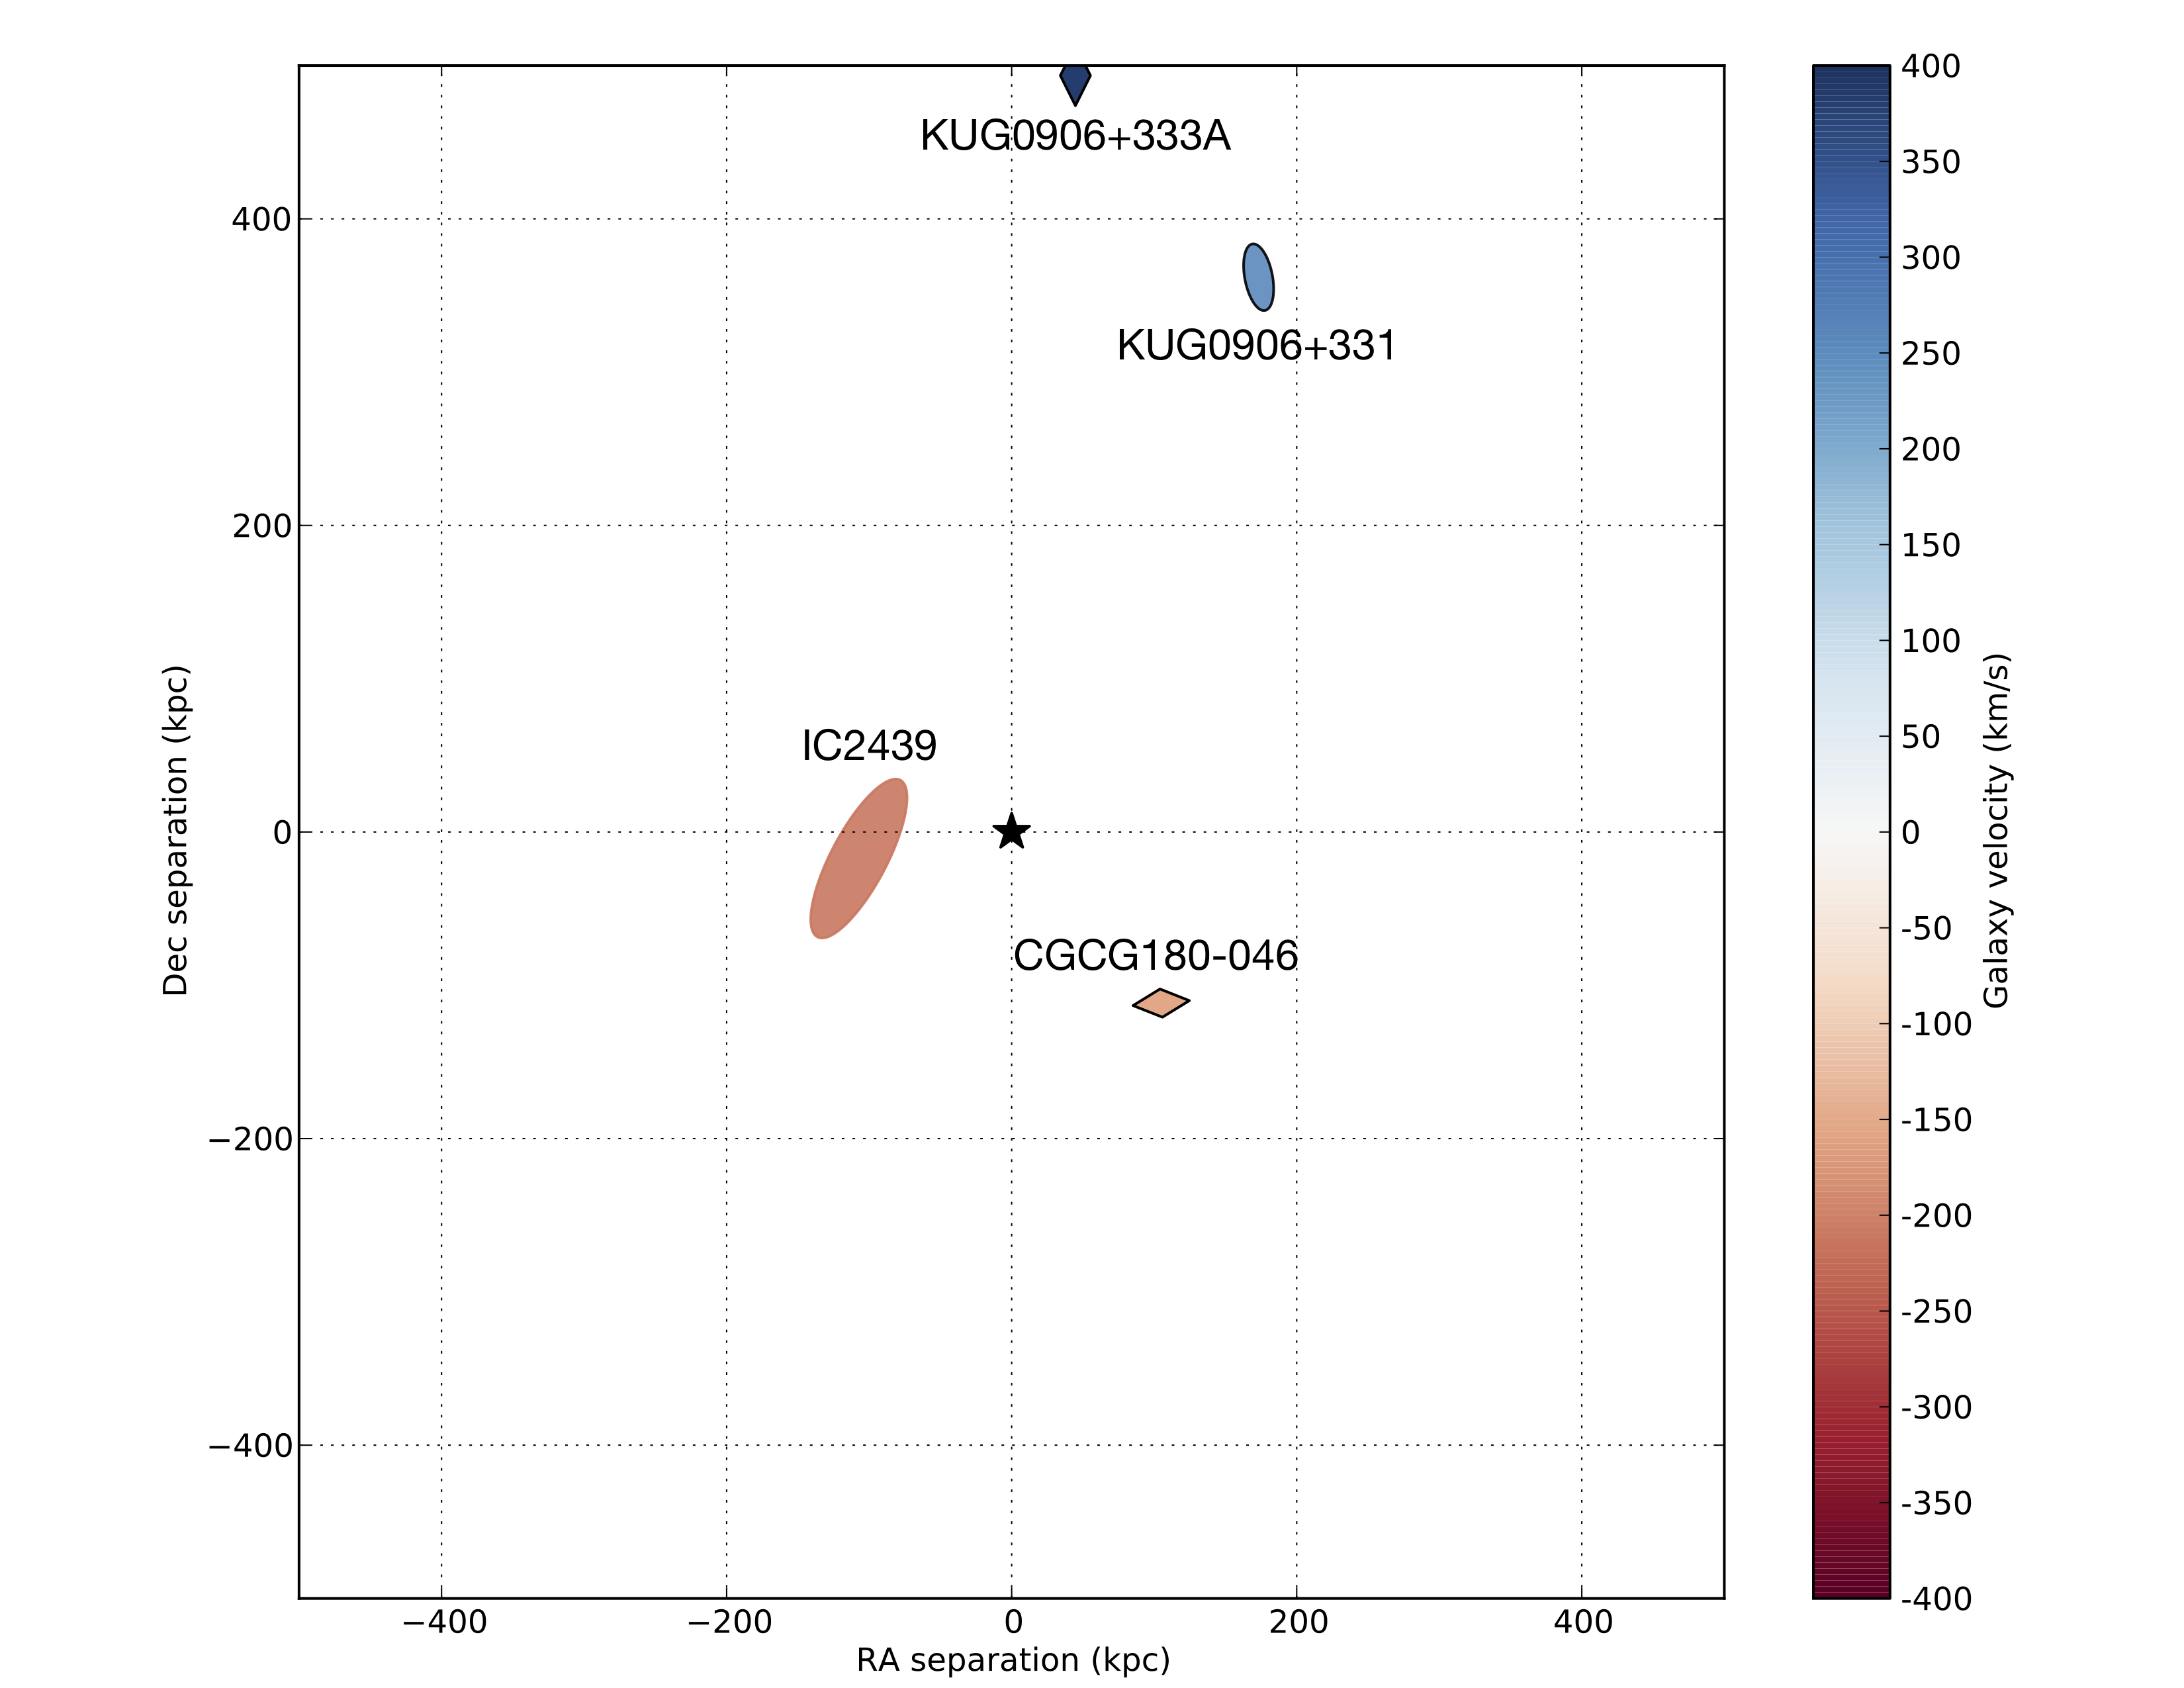
\includegraphics[width=\textwidth]{map_TON1009_4285_crop2_labels.png}
        \caption{}
    \end{subfigure}
  \caption{\small{a) An example Ly$\alpha$ line found in a sightline towards target TON1009 at 4295 km/s. b) A map of \textit{all} galaxies within a 500 kpc impact parameter target TON1009 sightline and with velocity ($cz$) within 400 km/s of absorption detected at 4295 km/s (central black star). The galaxy IC2439 ($v=4494$ km/s, inclination = $71^{\circ}$) can be unambiguously paired with the Ly$\alpha$ absorption feature at $v=4295$ km/s following our selection criteria ($\mathcal{L}_{IC2439} = 0.45$, many times larger than all other nearby galaxies). Note that the galaxy sizes have been scaled up by a factor of 10 in this figure.}}
%  \vspace{-10pt}
  \label{line}
%    \caption{Caption place holder}
\end{figure}


\begin{figure}[h!]
 \vspace{-5pt}
\centering
\begin{minipage}{.48\linewidth}
  \includegraphics[width=\linewidth]{W(impact_vir)_dif_cut_lighter.pdf}
  \captionof{figure}{Equivalent width of Ly$\alpha$ absorbers as a function of $\rho / R_{vir}$, the impact parameter to the associated galaxy normalized by the galaxy virial radius (French $\&$ Wakker 2016, in prep).}
  \label{virial}
\end{minipage}
\hspace{.01\linewidth}
\begin{minipage}{.48\linewidth}
  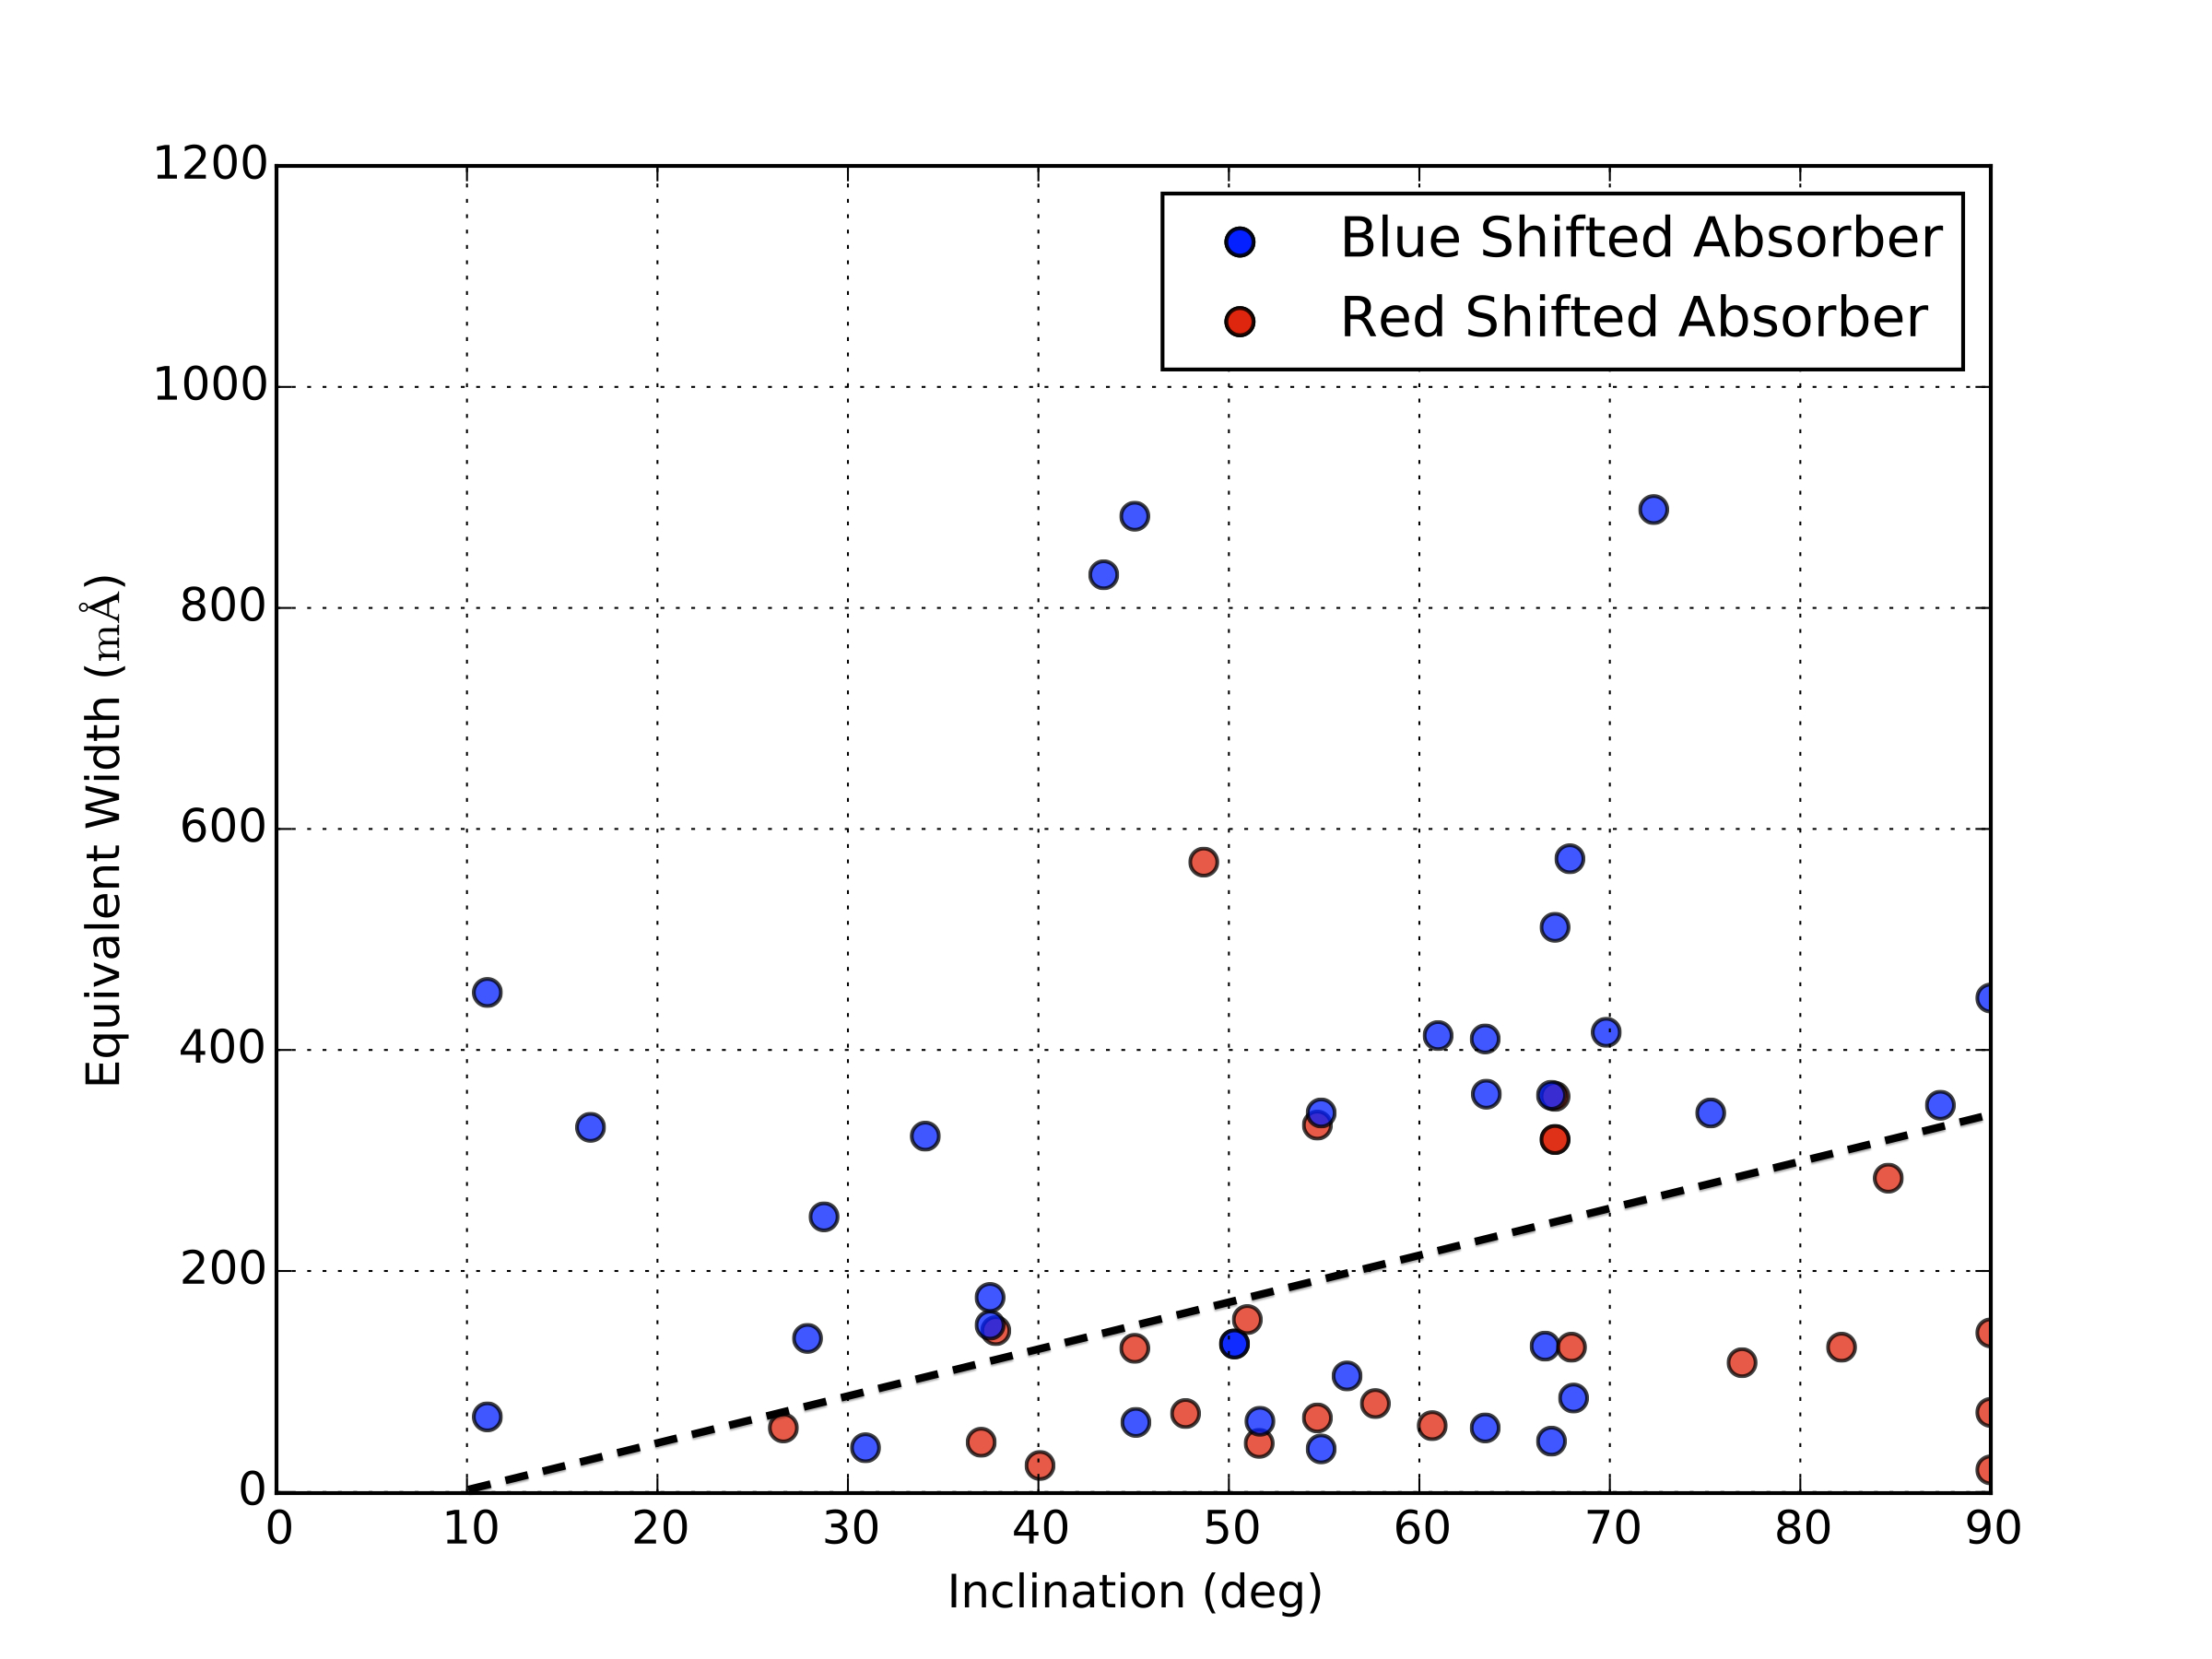
\includegraphics[width=\linewidth]{W(fancy_inclination)_dif_lighter_annotated.jpg}
  \captionof{figure}{Equivalent width of Ly$\alpha$ absorbers as a function of the inclination of the associated galaxy. The black dashed line highlights the dichotomy between red and blue shifted absorbers (French $\&$ Wakker 2016, in prep).}
  \label{dichotomy}
\end{minipage}
\end{figure}


\noindent \textbf{References: } Bowen, D.V., et al. 2002, ApJ, 580, 169; Carswell, B., et al. 2002, ApJ, 578, 43C; Cen, R. 2013, ApJ, 770, 139; Danforth, C.W., $\&$ Shull, J.M. 2008, ApJ, 679, 194D; Kacprzak, G.G., et al. 2011, MNRAS, 416, 3118; Kacprzak, G.G., et al. 2014, ApJ, 792L, 12K; Kim, T.S., et al. 2007, MNRAS, 382, 1657K; Lehner, N., et al. 2007, ApJ, 658, 680L; Mathes, N.L., et al. 2014, ApJ, 792, 128; Rudie, G.C., et al. 2012, ApJ,  750, 67; Savage, B.D. $\&$ Sembach, K.R. 1991, ApJ, 379, 245S; Steidel, C.C., et al. 2010, ApJ, 717, 289; Stewart, K.R., et al. 2011, ApJ, 738, 39; Stocke, J. T., et al. 2013, ApJ, 763, 148; Tumlinson, J., et al. 2013, ApJ, 777, 59T; Wakker B.P. \& Savage B.D. 2009, ApJs, 182, 378; Werk, J. K., et al. 2014, ApJ, 792, 8

%%%%%%%%%%%%%%%%%%%%%%%%%%%%%%%%%%%%%%%%%%%%%%%%%%%%%%%%%%%%%%%%%%%%%%%%%%%
%   2. ANALYSIS PLAN
%       (see Section 9.6 of the Call for Proposals)
%
%
\describearchival       % Do not delete this command.
% Enter your analysis plan here.

\noindent \textbf{\underline{1. Line Identifications and Measurements:}}

We will begin by aligning and combining multiple exposures to produce a single, clean spectrum. We then apply the line identification code, the mechanics of which are relatively simple and robust. First, we fit gaussian a profile to all spectral features above $2\sigma$ significance to determine their centroid wavelengths. Second, this list is fed into our algorithm, which produces IDs for each feature. We inspect each ID and make adjustments as needed. In this way each spectrum is both fit by machine and checked by eye, which minimizes miss-fits and machine artifacts. This will result in a dataset of all absorption lines with ID's, velocities, equivalent widths, and linewidth estimates.

Once ID'd, we carefully measure all spectral features in the $cz\le 10,000$ km/s redshift window. After fitting a low order (1st or 2nd) polynomial to line-free regions around each absorption line, we calculate the column density and estimate a linewidth using the apparent optical depth method (see Savage $\&$ Sembach 1991), as well as by making a Voigt profile fit using the VPFIT package (see Carswell et al. 2002, Kim et al. 2007).\\

\noindent \textbf{\underline{2. Galaxy-Absorber Matching:}}

Next, we correlate our galaxy dataset with the newly produced absorber dataset. This will produce matched absorber-galaxy systems based on our likelihood criteria. 

\textbf{New Nearby Galaxy Catalog:} Our nearby galaxy catalog contains over 108,000 galaxies, and is nearly complete to $\sim0.2 L^{\**}$ at $10,000$ km/s (progressively better towards lower redshifts). The data table contains the following entries for each galaxy: coordinates, redshift, heliocentric and Virgocentric flow corrected velocities, redshift-independent-distance, inclination, position angle, morphology, extinction, photometry, group association, and alternative galaxy names. NED makes an effort to homogenize these data, but we go further by preferentially using 2MASS $K_s$-band values for inclination, position angle, and diameter measurements. When these are not available, we scale measurements in other bands (e.g. SDSS $g$ and $r$) to the expected $K_s$-band values based on correlations between photometry bands. 2MASS values were chosen as it is an all-sky survey, and measurements are available for the majority of galaxies. Additionally, we calculate best-estimate B-band magnitudes and $L^{\**}$ values from the multitude of disparate photometry values included in NED. \\

%by normalizing all measurements of inclination, position angle, and diameter to 2MASS $K$-band values. 

\noindent \textbf{\underline{3. Interpretation:}}

With both the absorption line and nearby galaxy datasets in hand, we will investigate how Ly$\alpha$ equivalent width varies as a function of associated galaxy inclination, impact parameter, morphology, virial radius, azimuth angle, and system velocity with respect to absorption velocity. Particular attention will be paid to how these effects vary with proximity to the galaxies (i.e. within bins of velocity,  impact parameter, and likelihood), so that we can understand the CGM-galaxy connection and how it evolves across a range of scales. 

To address our original question, ``does the CGM follow the rotation direction and velocity of the associated galaxies?", we have secured Priority 1 time on the Southern African Large Telescope (SALT) to measure the rotation curves of 15+ galaxies with COS sightlines lying within $2R_{vir}$. With this data in hand we will compare the rotation and orientation of the galaxies with that of Ly$\alpha$ absorption detected in their halos, investigating if the Ly$\alpha$ absorbers tend to co-rotate with the direction of the gaseous disk, and if so, out to what distance.

% published in order as ground observations become available and IDing COS spectra progresses. The first will be the study of SALT rotation curves vs Ly$\alpha$ halo absorption, the second will be the full analysis of absorber properties as functions of galaxy properties. This second paper will also include an electronic data set containing all COS IDs, absorption line measurements, and galaxy associations.\\

%This catalog is complete to $\sim0.2 L^{\**}$ at $10,000$ km/s (and progressively better towards lower redshifts), making it the most complete, comprehensive and up-to-date nearby galaxy catalog in existence (to be published in 2016), and is key to allowing us to draw direct comparisons between the properties of the absorbers in the CGM and the properties of galaxies on a larger scale then ever before.\\

%%%%%%%%%%%%%%%%%%%%%%%%%%%%%%%%%%%%%%%%%%%%%%%%%%%%%%%%%%%%%%%%%%%%%%%%%%%

%   3. MANAGEMENT PLAN
%       (see Section 9.7 of the Call for Proposals)
%
%  Provide a concise, but complete, management plan. This plan will be used
%  by the review panels to assess the likely scale of the proposed research
%  program. Proposers should include a schedule of the work required to
%  achieve the scientific goals of the program, a description of the roles of the
%  PI, CoIs, postdocs, and students who will perform the work, and a plan to
%  disseminate the results to the community.
%
\budgetnarrative       % Do not delete this command. CALLS the Management Plan header in the Style File (IGNORE the command name of budgetnarrative
% Enter your management plan here.

\noindent \textbf{\underline{1) Line Identifications and Measurements: (5 months led by all team members)}}\\
\indent The time needed to ID a sightline can be as little as half an hour for an easy, low-redshift target, to several days for one at $z>1$; for the first 100 we have already completed, the median is $\sim 2$ hours. With all 3 team members contributing, we expect to easily complete the identification of 200 additional targets within 5 months.\\

\noindent \textbf{\underline{2) Galaxy-Absorber Matching: (1 months led by French)}}\\
\indent The likelihood algorithm and infrastructure for matching absorbers with galaxies is already in place from our pilot study. The first round of matching will not take long, but some additional time must be spent to inspect the results and discard occasional odd, or overly ambiguous systems. \\


\noindent \textbf{\underline{3) Interpretation and Publication: (9 months led by French and Wakker)}}\\
\indent Much of the analysis code required has also already been written for the pilot study, so only minor changes will need to be made here. Once the raw statistics and figures are produced, the majority of this time will be spent writing up the results. 

We plan to publish our results in a series of papers. First, the list of COS IDs and line measurements, as well as our new nearby galaxy catalog, will be published and made available electronically once this step is completed. Next, we will complete and publish our study of absorber properties as a function of galaxy properties (including new SALT rotation curves). Finally, with the robust statistics provided by our completed datasets, we plan to publish our results on the global CGM density profile and velocity fields in the nearby universe.


\end{document}          % End of proposal. Do not delete this line.
                        % Everything after this command is ignored.

